%% Compilar com: pdflatex RelatorioCLN.tex
%% Requer ceurart.cls (incluido nesta pasta; tambem em https://ctan.org/pkg/ceurart)
%% A imagem exemplo-resposta.png deve estar na mesma pasta.

\documentclass[]{ceurart}

\sloppy
\usepackage{listings}
\usepackage{graphicx}

\lstset{
  breaklines=true,
  basicstyle=\ttfamily\small,
  frame=single,
  backgroundcolor=\color[gray]{0.97},
  rulecolor=\color[gray]{0.80},
}

\begin{document}

\copyrightyear{2026}
\copyrightclause{Copyright for this paper by its authors.
  Use permitted under Creative Commons License Attribution 4.0
  International (CC BY 4.0).}

\conference{UBI 2025/26, Mestrado em Engenharia Informática, Computação em Linguagem Natural}

\title{Sistema Local de Perguntas e Respostas com \\ Retrieval-Augmented Generation: Llama~3.2, ChromaDB e Web Scraping}

\author{Enrico Nunes}[%
  email=enrico.nunes@ubi.pt,
]
\address{Universidade da Beira Interior, Covilhã, Portugal}

\begin{abstract}
Este relatório descreve a conceção e a implementação de um sistema local de
perguntas e respostas baseado em \emph{Retrieval-Augmented Generation} (RAG).
A partir de um único endereço Web definido pelo utilizador, o sistema faz
\emph{web scraping} do conteúdo, segmenta-o, gera \emph{embeddings} com um modelo
\emph{Sentence-Transformers} e indexa-os numa base vetorial \textbf{ChromaDB}
persistida em disco. As respostas são geradas pelo modelo \textbf{Llama~3.2},
servido localmente pelo \textbf{Ollama}, usando exclusivamente o contexto
recuperado---uma estratégia explícita de mitigação de alucinações. Todo o
processamento, com exceção da recolha inicial de dados, ocorre na própria
máquina, sem chamadas a APIs externas, cumprindo o requisito de operação
\emph{offline}. A solução foi desenvolvida num \emph{notebook} Jupyter organizado
em onze etapas sequenciais e fundamenta-se diretamente nas aulas teóricas de
Computação em Linguagem Natural da Universidade da Beira Interior.
\end{abstract}

\begin{keywords}
  Retrieval-Augmented Generation \sep
  Llama 3.2 \sep
  ChromaDB \sep
  Ollama \sep
  Sentence Transformers \sep
  Web Scraping
\end{keywords}

\maketitle

% ---------------------------------------------------------------------------
\section{Introdução}
% ---------------------------------------------------------------------------

O objetivo deste trabalho foi construir um sistema de perguntas e respostas
completamente \textbf{local} sobre uma fonte de conhecimento arbitrária da Web.
Em vez de enviar dados para serviços externos, toda a indexação, pesquisa
semântica e geração de resposta decorre na própria máquina.
A única etapa que necessita de ligação à Internet é a recolha inicial de
conteúdo (\emph{web scraping}); a partir desse momento, o sistema responde
\textbf{sem qualquer dependência de rede}.

Um sistema RAG combina duas fases: (1) a \emph{recuperação} dos excertos mais
relevantes para uma pergunta e (2) a \emph{geração} de uma resposta fundamentada
nesse contexto~\cite{gao2024rag}. Esta abordagem permite responder com base num
corpus específico---neste caso, uma página Web indexada---em vez de depender
apenas do conhecimento paramétrico do modelo de linguagem, reduzindo
o problema das \emph{alucinações}~\cite{ji2023hallucination}.

O sistema foi implementado num \emph{notebook} Jupyter, deliberadamente dividido
em etapas curtas e com lógica temporal, de modo a tornar transparente cada passo
do \emph{pipeline}. O código-fonte está disponível publicamente
em\footnote{\url{https://github.com/enriconunes/sistema-RAG-Local-Llama-ChromaDB}}.
Este relatório começa por contextualizar as ferramentas e conceitos centrais
(Secção~\ref{sec:fundamentos}), enquadra o trabalho nas aulas teóricas da unidade
curricular (Secção~\ref{sec:aulas}), descreve a arquitetura
(Secção~\ref{sec:arquitetura}) e detalha as onze etapas do
\emph{notebook} (Secção~\ref{sec:etapas}), terminando com uma demonstração real
do sistema, a declaração de utilização de IA generativa e as conclusões.

% ---------------------------------------------------------------------------
\section{Fundamentos e Ferramentas Centrais}
\label{sec:fundamentos}
% ---------------------------------------------------------------------------

Antes de descrever a implementação, importa contextualizar os temas que sustentam
o trabalho. Estes são, simultaneamente, os conceitos teóricos e as ferramentas
concretas que compõem o sistema.

\paragraph{Transformadores e modelos de linguagem.}
A arquitetura \emph{Transformer}, introduzida por Vaswani et
al.~\cite{vaswani2017attention}, substituiu a recorrência pelo mecanismo de
\emph{self-attention} e tornou-se a base de praticamente todos os modelos de
linguagem modernos. Sobre ela construiu-se o \textbf{BERT}~\cite{devlin2019bert},
um modelo bidirecional pré-treinado por \emph{masked language modeling}, que
popularizou as representações contextuais de texto. Estes dois trabalhos são a
fundação tanto dos modelos geradores quanto dos modelos de \emph{embeddings}
usados neste sistema.

\paragraph{Modelos de linguagem de grande escala e o Llama~3.2.}
Os \emph{Large Language Models} (LLM) são modelos \emph{Transformer} de grande
dimensão capazes de gerar texto fluente. Neste trabalho utiliza-se o
\textbf{Llama~3.2}, pertencente à família de modelos abertos da Meta descrita
em \emph{The Llama 3 Herd of Models}~\cite{llama3}. A escolha de um modelo aberto
é decisiva: permite executá-lo \textbf{localmente}, sem custos por chamada e sem
enviar dados para partes externas ao sistema. Essa execução local é assegurada pelo
\textbf{Ollama}~\cite{ollama}, um servidor que descarrega, gere e expõe modelos
de linguagem na própria máquina através de um \emph{endpoint} HTTP em
\texttt{localhost}.

\paragraph{Embeddings e recuperação semântica.}
A recuperação em RAG assenta em \emph{embeddings}: vetores numéricos que
posicionam textos com significado semelhante próximos uns dos outros. Em vez da
pesquisa por palavras-chave, usa-se \emph{dense retrieval}, onde a pergunta e os
documentos são projetados no mesmo espaço vetorial e comparados por similaridade.

\paragraph{Bases de dados vetoriais.}
Os \emph{embeddings} têm de ser armazenados e pesquisados de forma eficiente.
Para isso usa-se o \textbf{ChromaDB}~\cite{chromadb}, uma base de dados vetorial
de código aberto, orientada a aplicações de IA, que persiste os vetores em disco
(via SQLite) e permite recarregá-los posteriormente sem acesso à rede---uma
propriedade essencial para o modo \emph{offline}.

\paragraph{Retrieval-Augmented Generation e alucinações.}
O RAG~\cite{gao2024rag} articula recuperação e geração para fundamentar as
respostas em evidência textual concreta. O seu principal benefício é reduzir as
\emph{alucinações}---afirmações fluentes mas factualmente incorretas ou não
suportadas---um problema sistematicamente documentado na
literatura~\cite{ji2023hallucination}. Ao obrigar o modelo a responder apenas com
base no contexto recuperado, e a admitir quando a informação não está disponível,
o sistema torna-se mais fiável e auditável.

\paragraph{Orquestração e recolha de dados.}
A composição do \emph{pipeline} (recuperação, construção de \emph{prompt} e
geração) é feita com a \emph{framework} \textbf{LangChain}~\cite{langchain},
através da sua linguagem de composição declarativa (LCEL). A recolha inicial do
conteúdo Web é feita com \texttt{requests} e \textbf{Beautiful
Soup}~\cite{beautifulsoup}, que faz \emph{parsing} do HTML e extrai o texto
relevante.

% ---------------------------------------------------------------------------
\section{Enquadramento nas Aulas de Computação em Linguagem Natural}
\label{sec:aulas}
% ---------------------------------------------------------------------------

Todo o trabalho foi baseado nas aulas teóricas da unidade curricular de
\emph{Computação em Linguagem Natural} (UBI, MEI, 2025/26), lecionadas pelo
Prof. João Cordeiro. Em concreto, os temas deste projeto decorrem diretamente de
três aulas:

\begin{itemize}
  \item \textbf{Aula Teórica 09 --- \emph{Masked Language Models: BERT}.}
        Apresenta os modelos bidirecionais baseados em transformadores, as
        representações contextuais e a motivação para a recuperação de informação
        e para o RAG, incluindo a discussão das alucinações dos modelos de
        linguagem. Fundamenta os conceitos de \emph{embeddings} e de recuperação
        semântica usados no sistema.
  \item \textbf{Aula Teórica 10 --- \emph{Prompt Engineering + RAG}.}
        Introduz a engenharia de \emph{prompts}, o \emph{pipeline} de RAG
        (\emph{loading}, \emph{chunking}, \emph{embedding} e \emph{vector store}),
        a recolha de conteúdo da Web e a \emph{framework} LangChain. Corresponde
        à espinha dorsal da fase de ingestão deste trabalho.
  \item \textbf{Aula Teórica 11 --- \emph{RAG, LangChain, Indexing, Topic
        Modeling}.} Demonstra a utilização do LangChain com diferentes modelos e
        bases de dados, nomeadamente \textbf{Llama~3.2} e \textbf{ChromaDB}, a
        construção de cadeias LCEL, os \emph{loaders} e \emph{text splitters}, e
        ainda a modelação de tópicos com LDA. É a aula mais próxima da solução
        aqui apresentada.
\end{itemize}


% ---------------------------------------------------------------------------
\section{Arquitetura}
\label{sec:arquitetura}
% ---------------------------------------------------------------------------

A solução divide-se em dois fluxos bem delimitados, separados por uma fronteira
\emph{online}~/~\emph{offline}:

\begin{enumerate}
  \item \textbf{Ingestão} (executada uma vez, requer Internet): a partir de um
        \texttt{URL}, faz-se \emph{web scraping} do conteúdo, segmenta-se em
        \emph{chunks}, geram-se \emph{embeddings} e indexam-se na ChromaDB,
        persistida em disco.
  \item \textbf{Operação} (\emph{offline}, sem APIs): dada uma pergunta, o
        \emph{retriever} recupera os \emph{chunks} mais relevantes da base, que
        são injetados num \emph{prompt} e enviados ao Llama~3.2 (via Ollama) para
        produzir uma resposta ancorada e com indicação das fontes.
\end{enumerate}

Esta separação é central: depois de a base vetorial estar em disco, a fase de
operação não volta a aceder à rede, o que é demonstrado explicitamente na última
etapa do \emph{notebook} (modo \emph{offline}).

% ---------------------------------------------------------------------------
\section{As Onze Etapas do Sistema}
\label{sec:etapas}
% ---------------------------------------------------------------------------

O \emph{notebook} está organizado de forma sequencial. A \textbf{Etapa~0} é a
configuração centralizada; as \textbf{Etapas 1 a 11} constituem o \emph{pipeline}
propriamente dito, da verificação do ambiente até à operação \emph{offline}.
Descreve-se de seguida cada etapa, com a respetiva justificação técnica.

\subsection*{Etapa 0 --- Configuração}

Todos os parâmetros do sistema ficam reunidos num único bloco, para que mudar de
fonte de conhecimento se resuma a alterar o \texttt{URL} e reexecutar o
\emph{notebook}.

\begin{lstlisting}
URL             = "https://pt.wikipedia.org/wiki/Processamento_de_linguagem_natural"
OLLAMA_MODEL    = "llama3.2"
OLLAMA_BASE_URL = "http://localhost:11434"
EMBEDDING_MODEL = "sentence-transformers/paraphrase-multilingual-MiniLM-L12-v2"
CHROMA_DIR      = "chroma_db"   # persistencia em disco
CHUNK_SIZE      = 1000
CHUNK_OVERLAP   = 100
TOP_K           = 4             # chunks recuperados por pergunta
\end{lstlisting}

\subsection*{Etapa 1 --- Verificação do ambiente}

Antes de avançar, a função \texttt{verificar\_ollama()} interroga o servidor
local (\emph{endpoint} \texttt{/api/tags}) para confirmar que o Ollama está
acessível e que o modelo \texttt{llama3.2} está descarregado. Trata-se de um
processo local, não de uma API remota. Esta verificação prévia evita falhas
obscuras mais à frente e dá ao utilizador instruções claras de correção.

\subsection*{Etapa 2 --- Web Scraping}

É a \textbf{única} etapa que necessita de Internet. A função
\texttt{extrair\_conteudo(url)} faz o pedido HTTP com \texttt{requests} e analisa
o HTML com Beautiful Soup~\cite{beautifulsoup}, removendo elementos sem valor
informativo (\texttt{script}, \texttt{style}, \texttt{nav}, \texttt{footer},
etc.), privilegiando o corpo principal do artigo e normalizando espaços e linhas.

\begin{lstlisting}
soup = BeautifulSoup(resp.text, "html.parser")
for tag in soup(["script","style","nav","footer","header","aside","noscript","form"]):
    tag.decompose()
principal = soup.find("main") or soup.find("article") or soup.body or soup
texto = principal.get_text(separator="\n")
\end{lstlisting}

\subsection*{Etapa 3 --- Chunking (segmentação)}

O texto extraído é demasiado grande para ser usado de uma só vez, pelo que é
dividido em segmentos menores com o \texttt{RecursiveCharacterTextSplitter}
(\texttt{chunk\_size=1000}, \texttt{chunk\_overlap=100}).
A sobreposição (\emph{overlap}) preserva o contexto na fronteira entre
\emph{chunks}, evitando que informação relevante fique artificialmente cortada.
A cada \emph{chunk} é atribuído um identificador, para mais tarde citar a
proveniência da resposta.

\subsection*{Etapa 4 --- Embeddings locais}

Cada \emph{chunk} é convertido num vetor que captura o seu significado, com um
modelo \emph{Sentence-Transformers} executado \textbf{localmente}
(\texttt{HuggingFaceEmbeddings}). Os vetores são normalizados, o que torna a
similaridade do cosseno equivalente ao produto interno.

\subsection*{Etapa 5 --- Indexação no ChromaDB}

Os \emph{chunks} e respetivos vetores são guardados na ChromaDB com
\texttt{Chroma.from\_documents(...)}, que cria a coleção e persiste tudo em disco
via SQLite~\cite{chromadb}. Depois desta etapa, a base pode ser recarregada
\emph{offline} (Etapa~11), sem reprocessar a página.

\begin{lstlisting}
vector_store = Chroma.from_documents(
    documents=chunks, embedding=embeddings,
    collection_name=COLLECTION_NAME, persist_directory=CHROMA_DIR,
)
\end{lstlisting}

\subsection*{Etapa 6 --- Retriever}

A partir da base cria-se um \emph{retriever} com
\texttt{as\_retriever(search\_kwargs=\{"k": TOP\_K\})}, que devolve os \texttt{k}
\emph{chunks} mais semelhantes a cada pergunta, por similaridade no espaço de
\emph{embeddings}. O \emph{notebook} mostra explicitamente \emph{que} excertos
são recuperados para uma consulta de exemplo---uma transparência que ajuda a
compreender (e a defender) cada resposta.

\subsection*{Etapa 7 --- Modelo de linguagem local (Ollama + Llama~3.2)}

Carrega-se o Llama~3.2~\cite{llama3} através do \texttt{ChatOllama}. Define-se \texttt{temperature=0} para tornar as respostas determinísticas e
menos propensas a invenção.

\subsection*{Etapa 8 --- Cadeia RAG (LCEL)}

Compõe-se o \emph{pipeline} em LCEL~\cite{langchain}, ligando \emph{retriever},
\emph{prompt}, modelo e \emph{parser} de saída:

\begin{lstlisting}
rag_chain = (
    {"context": retriever | formatar_docs, "question": RunnablePassthrough()}
    | prompt | llm | StrOutputParser()
)
\end{lstlisting}

O \emph{prompt} de sistema é o coração da estratégia anti-alucinação: instrui o
modelo a responder \textbf{exclusivamente} com base no contexto e, se a
informação não constar, a devolver exatamente \emph{``Não encontrei essa
informação no conteúdo indexado.''}~\cite{ji2023hallucination}.

\subsection*{Etapa 9 --- Perguntas e Respostas}

A função \texttt{perguntar()} executa a cadeia e apresenta a resposta
\textbf{acompanhada das fontes} (os \emph{chunks} efetivamente utilizados),
seguindo a ideia de citação de proveniência. Mostrar as fontes é o que distingue
uma resposta verificável de uma afirmação opaca.

\subsection*{Etapa 10 --- Demonstração anti-alucinação}

Esta etapa contrasta, para a mesma pergunta, duas respostas: a do \textbf{modelo
sozinho} (que responde a partir da memória paramétrica e pode inventar) e a do
\textbf{sistema com RAG} (que se ancora no conteúdo indexado e, na ausência de
evidência, recusa responder). É a materialização prática do problema das
alucinações.

\subsection*{Etapa 11 --- Modo Offline}

Para provar o requisito de operação sem Internet, a função
\texttt{carregar\_sistema\_offline()} \textbf{recarrega a ChromaDB já persistida
em disco} (sem \emph{scraping} nem APIs) e reconstrói a cadeia de resposta. É
possível desligar a rede e executar apenas esta célula, obtendo na mesma
respostas fundamentadas.

\subsection{Demonstração: comportamento indexado vs.\ não indexado}

A Figura~\ref{fig:exemplo} mostra o sistema em funcionamento real, com a fonte
indexada sobre Processamento de Linguagem Natural (PLN). Ilustra os dois
comportamentos que resumem todo o trabalho:

\begin{itemize}
  \item \textbf{Pergunta não indexada} (\emph{``qual é o atual presidente de
        portugal?''}): como a resposta não consta do conteúdo recuperado, o
        sistema \textbf{recusa-se a inventar} e devolve \emph{``Não encontrei essa
        informação no conteúdo indexado.''}.
  \item \textbf{Pergunta indexada} (\emph{``o que é PNL''}): o sistema produz uma
        resposta correta e fundamentada no material indexado, definindo o
        Processamento Natural de Linguagem como área da Computação dedicada a
        compreender e gerir a linguagem humana.
\end{itemize}

Este contraste é a evidência central de que o sistema cumpre o seu propósito:
\textbf{responde quando tem suporte na fonte e admite quando não tem}, reduzindo
as alucinações~\cite{ji2023hallucination,gao2024rag}.

\begin{figure}[h]
  \centering
  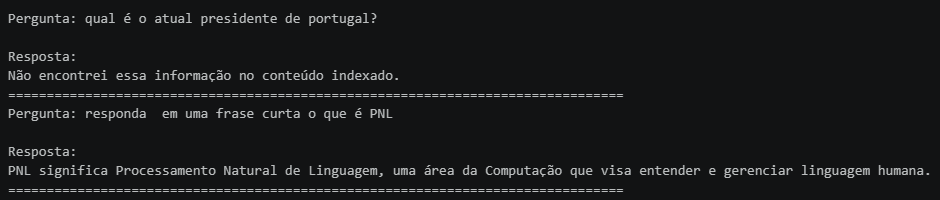
\includegraphics[width=\linewidth]{exemplo-resposta.png}
  \caption{Funcionamento real do sistema: uma pergunta \emph{não indexada} é
  recusada (em cima) e uma pergunta \emph{indexada} é respondida com base no
  conteúdo (em baixo).}
  \label{fig:exemplo}
\end{figure}

% ---------------------------------------------------------------------------
\section{Utilização de IA Generativa no Desenvolvimento}
% ---------------------------------------------------------------------------

Na preparação deste trabalho, o autor recorreu a modelos de linguagem de grande
escala como auxílio na organização de conteúdos, na geração e revisão de código,
na elaboração de rascunhos iniciais e na revisão linguística do texto. Todo o
conteúdo produzido com recurso a estas ferramentas foi subsequentemente revisto
e validado pelo autor, que assegurou o seu rigor técnico e coerência académica e
assume plena responsabilidade pelo conteúdo final do presente trabalho.

% ---------------------------------------------------------------------------
\section{Conclusão}
% ---------------------------------------------------------------------------

Implementou-se um sistema RAG \textbf{completamente local}, capaz de responder a
perguntas em linguagem natural sobre uma página Web indexada, sem qualquer
chamada a APIs em operação e com funcionamento \emph{offline} após a ingestão. A
combinação de \emph{web scraping}, \emph{Sentence-Transformers}, ChromaDB,
LangChain e Llama~3.2 (via Ollama) reproduz fielmente a \emph{stack} ensinada nas
aulas de CLN da Universidade da Beira Interior, substituindo apenas os componentes baseados em API pelos seus
equivalentes locais.

A decisão técnica mais relevante foi ancorar a geração no contexto recuperado e
expor sempre as fontes, o que ataca diretamente o problema das
alucinações~\cite{ji2023hallucination}: o sistema responde com fundamento ou
admite explicitamente a ausência de informação. A separação clara entre ingestão
e operação permitiu, ainda, demonstrar de forma inequívoca o requisito de
funcionamento sem Internet.

Como trabalho futuro, identificam-se três direções alinhadas com as aulas:
combinar recuperação densa com pesquisa esparsa (BM25) numa abordagem híbrida;
acrescentar \emph{reranking} dos \emph{chunks} antes da geração; e indexar
múltiplas fontes (várias páginas ou PDFs), eventualmente caracterizando o corpus
com modelação de tópicos (LDA).

% ---------------------------------------------------------------------------
\begin{thebibliography}{11}

\bibitem{vaswani2017attention}
A. Vaswani, N. Shazeer, N. Parmar, J. Uszkoreit, L. Jones, A. N. Gomez,
L. Kaiser, and I. Polosukhin,
\textit{Attention Is All You Need},
Advances in Neural Information Processing Systems (NeurIPS), 2017.
\url{https://arxiv.org/abs/1706.03762}

\bibitem{devlin2019bert}
J. Devlin, M.-W. Chang, K. Lee, and K. Toutanova,
\textit{BERT: Pre-training of Deep Bidirectional Transformers for Language
Understanding},
Proceedings of NAACL-HLT, 2019.
\url{https://arxiv.org/abs/1810.04805}

\bibitem{llama3}
A. Grattafiori et al. (Llama Team, AI @ Meta),
\textit{The Llama 3 Herd of Models},
arXiv preprint arXiv:2407.21783, 2024.
\url{https://arxiv.org/abs/2407.21783}

\bibitem{gao2024rag}
Y. Gao, Y. Xiong, X. Gao, K. Jia, J. Pan, Y. Bi, Y. Dai, J. Sun, M. Wang,
and H. Wang,
\textit{Retrieval-Augmented Generation for Large Language Models: A Survey},
arXiv preprint arXiv:2312.10997, 2023.
\url{https://arxiv.org/abs/2312.10997}

\bibitem{ji2023hallucination}
Z. Ji, N. Lee, R. Frieske, T. Yu, D. Su, Y. Xu, E. Ishii, Y. J. Bang,
A. Madotto, and P. Fung,
\textit{Survey of Hallucination in Natural Language Generation},
ACM Computing Surveys, vol.~55, no.~12, 2023.
\url{https://arxiv.org/abs/2202.03629}

\bibitem{karpukhin2020dpr}
V. Karpukhin, B. O\u{g}uz, S. Min, P. Lewis, L. Wu, S. Edunov, D. Chen,
and W. Yih,
\textit{Dense Passage Retrieval for Open-Domain Question Answering},
Proceedings of EMNLP, 2020.
\url{https://arxiv.org/abs/2004.04906}

\bibitem{reimers2020multilingual}
N. Reimers and I. Gurevych,
\textit{Making Monolingual Sentence Embeddings Multilingual using Knowledge
Distillation},
Proceedings of EMNLP, 2020.
\url{https://arxiv.org/abs/2004.09813}

\bibitem{ollama}
Ollama,
\textit{Ollama: Get up and running with large language models locally},
2024.
\url{https://ollama.com}

\bibitem{chromadb}
Chroma,
\textit{Chroma: the open-source AI application database},
2024.
\url{https://www.trychroma.com}

\bibitem{langchain}
LangChain,
\textit{LangChain Documentation},
2024.
\url{https://python.langchain.com}

\bibitem{beautifulsoup}
L. Richardson,
\textit{Beautiful Soup Documentation},
2024.
\url{https://www.crummy.com/software/BeautifulSoup/}

\end{thebibliography}

\end{document}
